\chapter{Preliminaries and necessary background}
\label{chapter:background}
\newtheorem{theorem}{Theorem}
In this chapter we present the necessary background that the reader should have in order to proceed through the next two chapters, which are the core of this work. Here, we show the analysis done separately in graph kernels and in random features. However, we show our analysis combining these different notions in one algorithm in the next chapter.
\section{Kernel trick and random features}

\subsection{Kernel trick}
Kernel trick promotes the use of  positive semi-definite kernels $\mathcal{K}(x,x')$ in learning models as a similarity function between data points $(x,x')$. Where having $\mathcal{D}$ as the set of all possible data points, a function $\mathcal{K}:\mathcal{D}\times\mathcal{D}\mapsto\mathbb{R}$ is said to be a positive semi-definite kernel if:
\begin{itemize}
    \item $\forall (x,x')\in\mathcal{D}\times\mathcal{D}, \mathcal{K}(x,x')=\mathcal{K}(x',x)$
    \item $\forall n\in \mathbb{N}, \forall \alpha_1,\ldots,\alpha_n\in \mathbb{R},\forall x_1,\ldots,x_n\in \mathcal{D},\sum_{i,j}^n\alpha_i\alpha_j\mathcal{K}(x_i,x_j)\geq 0$
\end{itemize}
We show now how kernels can be incorporated within learning models and how that is useful to learn more complex functions. To do that let's consider the specific case when $\mathcal{D}=\mathbb{R}^d; d\in\mathbb{N}$, and let $(\mathbf{X},\mathbf{Y})$ be a labeled dataset of size $n$ with $\mathbf{X}\in \mathbb{R}^{n\times d} $ and for simplicity $\mathbf{Y}\in \{-1,1\}^n$, which is referred to as 2-classes dataset. Many of the learning models designed to solve this problem, like support vector machine and perceptron binary classifier, rely on the inner product as a measure of similarity between data points, as their output has the following formula \citep{inner_product}:
\begin{equation}
\label{eq:inner_product}
 \hat{y}(\mathbf{x})=sign\{\sum_{i=1}^n\alpha_iy_i\mathbf{x}_i^T\mathbf{x}\}; ~~~\forall i, (\mathbf{x}_i,y_i)\in (\mathbf{X,Y}),\alpha_i\in \mathbb{R}
\end{equation}

The values $[\alpha_i]_{i=1}^n$ in Eq. \ref{eq:inner_product} are optimized based on the dataset $(\mathbf{X,Y})$ by the learning algorithm. The intuition behind Eq. \ref{eq:inner_product} is that the output class for every new data point $x$ is expected to be the same class of nearby points in the input set $\mathcal{D}$. This is achieved by introducing the inner product $\mathbf{x}_i^T\mathbf{x}$ to control how much the class $y_i$ contributes in the output $\hat{y}(\mathbf{x})$. The parameters $[\alpha_i]_{i=1}^n$ controls how strongly can the train data point $x_i$ affect other neighbor points, and they mainly depend on how both classes are distributed in the input set $\mathcal{D}$, and on how much the dataset $(\mathbf{X,Y})$ is noisy. 
\begin{figure}[H]
\centering
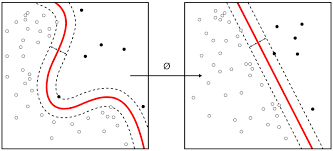
\includegraphics[scale=0.5]{LatexDiss/Dissertation/figs/svm.png}
\caption[The case where classes aren't separable using linear boundary]{The left figure shows a case where the input data in their original space are not separable by a linear boundary. The right figure shows the same data transformed to a new space using a lifting function \o, and we can see that different classes are now separable  using linear boundary.}
%Source:
\label{fig:SVM_boundaries}
\end{figure}
However, with Eq. \ref{eq:inner_product} can be rewritten as $\hat{y}(\mathbf{x})=sign\{\textbf{x}^T(\mathbf{X}^T~diag([\alpha]_{i=1}^n)~\mathbf{Y})\}$, where $diag([\alpha]_{i=1}^n)$ is the diagonal square matrix whose eigenvalues are $[\alpha]_{i=1}^n$, and $\mathbf{X}$ are the data points in the dataset. To get the decision boundary of such models we solve $\textbf{x}^T\textbf{q}=0$, where $\textbf{q}=(\mathbf{X}^T~diag([\alpha]_{i=1}^n)~\mathbf{Y})\in\mathbb{R}^d$, so what we get is that it is an equation of a hyper-plane in the input space $\mathbb{R}^d$, and we refer to this as a linear decision boundary. The question here is what if the the two classes are not separable by a hyper-plane as shown in Fig. \ref{fig:SVM_boundaries}. One common solution to this problem is to map the data points from $\mathbb{R}^d$ to another space $\mathbb{R}^m$  through a proper mapping function \o~such that classes become separable with a linear decision boundary in $\mathbb{R}^m$.Then we can apply the same learning models specified in Eq. \ref{eq:inner_product} but on the transformed data. Let's consider for example the dataset shown in Fig. \ref{fig:polynomial_kernel},  we can use the following mapping function \o$:(x_1,x_2)\mapsto (\sqrt{2}x_1x_2,x_1^2,x_2^2)$ to move from $\mathbb{R}^2$ on the left where data are not linearly separable to $\mathbb{R}^3$ on the right where they are.
\begin{figure}[H]
\centering
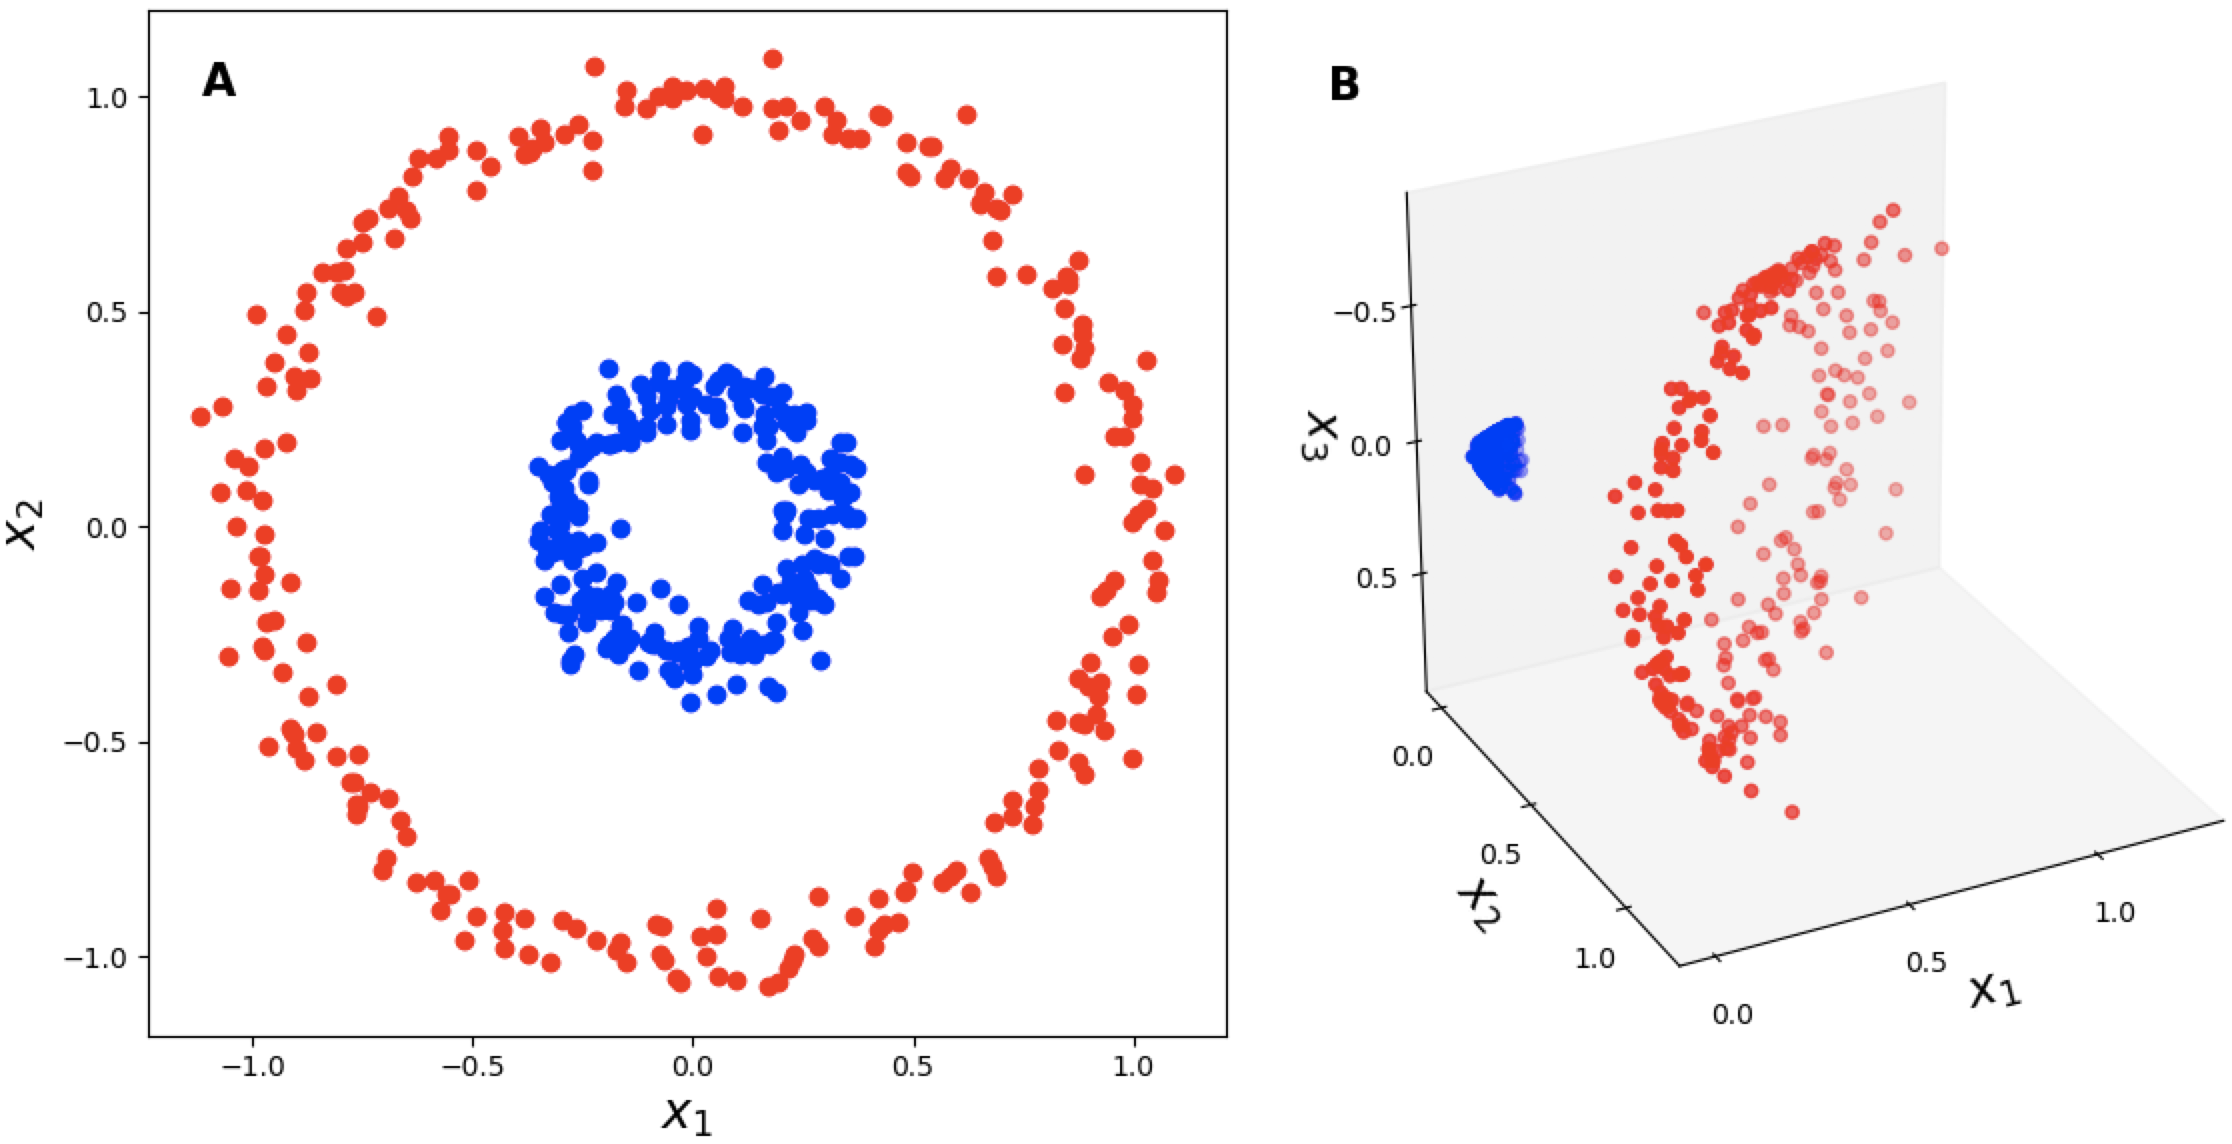
\includegraphics[scale=0.25]{LatexDiss/Dissertation/figs/poly_kenrnel.png}
\caption[Lifting data to a higher-dimension space to get linearly separable classes]{ Using the mapping function \o$:(x_1,x_2)\mapsto (\sqrt{2}x_1x_2,x_1^2,x_2^2)$ to map the data on the left in $\mathbb{R}^2$ to $\mathbb{R}^3$ where they are linearly separable}
%Source:
\label{fig:polynomial_kernel}
\end{figure}
Now the role of kernels can tackled here, but first we state the key theorem that justifies what follows.
\begin{theorem}[Mercer theorem]
To every positive semi-definite kernel $\mathcal{K}:\mathbb{R}^d\times \mathbb{R}^d\mapsto \mathbb{R}$, there exists a Hilbert space $\mathbb{H}$ and a feature map $\phi:\mathbb{R}^d\mapsto\mathbb{H}$ such that for all $x,x'\in\mathbb{R}^d$ we have: 
\begin{equation}
\label{eq:kernel_main_equation}
    \mathcal{K}(\mathbf{x},\mathbf{x}')=<\phi(\mathbf{x}),\phi(\mathbf{x}')>_\mathbb{H}
\end{equation}
where $<\phi(\mathbf{x}),\phi(\mathbf{x}')>_\mathbb{H}$ is the inner product defined in $\mathbb{H}$.
\end{theorem}
This theorem state that replacing the inner product \textbf{$\mathbf{x}_i^T\mathbf{x}$} in Eq. \ref{eq:inner_product} by a positive semi-definite kernel $\mathcal{K}(\mathbf{x},\mathbf{x}')$ is equivalent to implicitly map the data from the original input space $\mathcal{D}$ to another feature space $\mathbb{H}$ and then apply the classical inner product learning models. This is important because using such kernels, it is not important to know the implicit mapping function $\phi$ nor the new feature space $\mathbb{H}$. Instead, it is sufficient to evaluate the kernel for pairs of data points in the original input space $\mathcal{D}$. Indeed, that has two main advantages:
\begin{itemize}
    \item Kernels allow us to transform data to a new Hilbert space of very high or even infinite dimensionality, which can make the learning model able to represent more complex functions. This is not possible with the explicit mapping.
    \item Kernels are computationally cheaper, since they save the time required to compute the explicit co-ordinates of the data in the new feature space by directly calculate the inner product between the transformed data.
\end{itemize}
To better illustrate these benefits, we take the Gaussian kernel as an example, where:
\begin{equation}
\label{eq:Guassian_kernel}
    \mathcal{K}_{G}(\mathbf{x},\mathbf{x}')=exp(-\frac{\left \| \mathbf{x}-\mathbf{x}'\right\|^2}{2\sigma^2})
\end{equation}
where $\sigma$ is called the bandwidth parameter of the kernel. The lifting function $\phi_G$ of this kernel is located in a Hilbert space of infinite dimension, but the kernel can be easily evaluated for any pair $(\mathbf{x},\mathbf{x}')\in \mathcal{D}=\mathbb{R}^d$.\newline
Despite kernel methods, also referred to as kernel machines, have the previous advantages, they still have two drawbacks:
\begin{itemize}
    \item Since for most kernels we have access only to evaluate the kernel on pairs of data points, then for a dataset $(\mathbf{X},\mathbf{X})$ of size $n$, we need $O(n^2)$ memory entries to compute what is called Gram matrix. Where the $(i,j)_{th}$ entry equals the kernel between points $(\mathbf{x_i,x_j})\in \mathbf{X}$.
    \item Even that most kernels are designed so that they can be evaluated in polynomial time in the dimensionality of the input space $\mathcal{D}$, still some of the efficient kernels needs exponential time in the same dimensionality \citep{graphlet_kernel}.
\end{itemize}
To overcome these disadvantages, random feature projections discussed in the next section is a technique developed to approximate these kernels with less computational time and less memory storage.

\subsection{Random features}
Random features is a method developed to approximate kernel machines whose computational time  scales exponentially in the input dimensionality, and of course the goal is to reduce this time.   The idea is that instead of considering the true lifting function $\phi$ in Eq. \ref{eq:kernel_main_equation}, we explicitly map the data points to an Euclidean space of low dimensionality. This mapping is done using an appropriate randomized feature map $\varphi:\mathcal{D} \xrightarrow{}\mathbb{R}^m$. Then we approximate the kernel of two data points $x, x'$ by the inner product of their random features:
\begin{equation}
\label{eq:approx_RF}
\mathcal{K}(x,x')=<\phi(x),\phi(x')> \approx \varphi(x)^*\varphi(x')
\end{equation}
Considering this approximation, we can transform the input with $\varphi$ and then apply a fast linear learning method as in Eq. \ref{eq:inner_product} to have a similar learning power as the original non-linear kernel machine. In what follows, random Fourier features method to construct the random mapping function $\varphi$ is presented.
\begin{theorem}[Bochner's theorem]
A continuous and shift-invariant kernel $\mathcal{K}(x,x')=\mathcal{K}(x-x')$ on $\mathbb{R}^d$ is positive definite if and only if $\mathcal{K}(\delta)$ is the Fourier transform of a non-negative measure.
\end{theorem}
Direct consequence, we can easily scale a shift-invariant kernel so that its Fourier transform $p(w)$ is a correct probability distribution, since it is non-negative measure and integral-bounded function, and we write:
\begin{equation}
\label{Fourier integral}
\mathcal{K}(x-x')=\int_{\mathbb{R}^d}p(w)e^{jw^T(x-x')}dw=E_w[e^{jw^Tx}{e^{jw^Tx'}}^*]
\end{equation}
Both $p(w)$ and $\mathcal{K}(\delta)$ are real-valued functions, thus from Eq.~\ref{Fourier integral} one can prove that:
\begin{equation}
\label{real Fourier integral}
\mathcal{K}(x-x')=\int_{\mathbb{R}^d}p(w)cos({w^T(x-x')})dw=E_w[\xi_w(x)\xi_w(x')]
\end{equation}
where $\varphi_w(x)=\sqrt{2}cos(w^Tx+b)$ such that $w$ is drawn from $p(w)$ and b is drawn uniformly from $[0,2\pi]$.\newline
As a result, $\ \xi_w(x)\xi_w(x')$ is an unbiased estimate of $\mathcal{K}(x,x')$. Moreover, we can achieve lower variance estimation to the expectation (Eq. \ref{real Fourier integral}) by averaging $m$ instances of the estimator with different random frequencies $w$, \emph{i.e.} the low-variance estimator can be written as: $\varphi(x)^T\varphi(x')=\frac{1}{m} \Sigma_{j=1}^m \xi_{w_j}(x)\xi_{w_j}(x')$ where frequencies $w_j$ are identically and independently drawn from $p(w)$. This estimator and based on Hoeffding's inequality guarantees exponentially fast convergence in $m$ between $\varphi(x)^T\varphi(x')$ and the kernel true value:
\begin{equation}
    Pr(|\varphi(x)^T\varphi(x')-\mathcal{K}(x,x')|\geq\epsilon)\leq2e^\frac{-m\epsilon^2}{4};~~~ \forall \epsilon >0
\end{equation}
To better illustrate that, we consider the Gaussian kernel in Eq. \ref{eq:Guassian_kernel} as an example. This kernel is a function of the difference between both input points $\mathcal{K}_G(x,x')=f(x-x')$ and it is a positive semi-definite kernel. If we multiply this kernel with the constant $\frac{1}{2\pi}^d$ where $d$ is the dimensionality of the input data, then its Fourier transformation is a correct probability distribution:
\[p(w)=FT\big(\mathcal{K}_G(\delta)\big)(w)=(\frac{\sigma^2}{2\pi})^\frac{d}{2}e^{-\frac{\sigma^2\|w\|^2}{2}}\]
Where $\delta\in\mathbb{R}^d$ and $w\in\mathbb{R}^d$.

\section{Graph kernels}
 We first introduce  necessary notations related to graph definition and graph kernels.\newline $F=(\mathcal{V}_F,\mathcal{E}_F)$ is said to be a subgraph (graphlet) of $\mathcal{G}$ and we write $F\sqsubseteq \mathcal{G}$, if and only if there exist an injective function $\mathcal{M}:\mathcal{V}_F\xrightarrow{} \mathcal{V}$ such that $(u,u')\in \mathcal{E}_F \Leftrightarrow{(\mathcal{M}(u),\mathcal{M}(u'))\in \mathcal{E}}$.\newline
Any edge $(u_i, u_i)$ is called a self loop. In a general graph two vertices $u_i$ and $u_j$ may be connected by more than
one edge. A simple graph is a graph with no self loops
or multiple edges. Here we always consider simple graphs.\newline
A simple graph can equivalently be represented by an adjacency matrix $\mathbf{A}$ of size $v \times v$. The $(i,j)-th$ entry of $\mathbf{A}$ is 1 if an edge $(u_i, u_j)$ exists and zero otherwise.\newline
Two graphs $\mathcal{G}=(\mathcal{V},\mathcal{E})$ and $\mathcal{G'}=(\mathcal{V'},\mathcal{E'})$ are isomorphic and we write $\mathcal{G}'\cong \mathcal{G}$ if there exists a bijective function $\mathcal{M}:\mathcal{V}\xrightarrow{} \mathcal{V}'$ such that $(u_i,u_j)\in \mathcal{E}$ iff $(\mathcal{M}(u_i),\mathcal{M}(u_j))\in \mathcal{E}'$.

\subsection{Convolutional graph kernels}
Traditional kernel machines approach problems with vector-valued input data, where they compare different data points $(x,x' \in \mathcal{R}^d)$ using the difference between correspondent pairs of vector entries. Based on that, these kernels are imperfect to be used with graphs, since the graph structure is permutation invariant, i.e. isomorphic graphs have different adjacency matrices but they represent the same structure. So in this case distance-kernels between graph representation vectors (adjacency matrices for example ) are not a good choice. As a result it is necessary to measure distance between graphs in ways that are  permutation invariant as well. Here the concept of isomorphism is critical in learning algorithms on graphs,  not only because there is no known polynomial-time algorithm for testing graph isomorphism (except for graphs with specific structures), but isomorphism is also too strict for learning in a similar way to learning with equality operator \citep{kriege_graph_kernels}. \newline
Most of graph kernels developed for graph learning problems are convolution kernels, where given two graphs, the trick is to divide each into smaller subgraphs and then to pairwise compute the kernel between the resulted subgraphs.
\newtheorem{definition}{Definition} 
\begin{definition}[Convolution Kernel]
let $\mathcal{R}=\mathcal{R}_1\times...\times \mathcal{R}_d$ denote a space of components such that a composite object $X\in \mathcal{X}$ decomposes into elements of $\mathcal{R}$. Let $R:\mathcal{R}\xrightarrow{}\mathcal{X}$ denote the mapping from components to objects, such that $R(x)=X$ iff the components $x\in \mathcal{R}$ make up the object $X\in \mathcal{X}$, and let $R^{-1}(X)=\{x\in\mathcal{R}:R(x)=X\}$. then, the R-convolution kernel is:
\begin{equation}
\label{eq:conolutional_kernels}
    K_{CV}(X,Y)=\sum_{x\in R^{-1}(X)}~\sum_{y\in R^{-1}(Y)}~\underbrace{\prod_{i=1}^{d}k_i(x_i,y_i)}_{k(x,y)}
\end{equation}
with $k_i$ is a kernel on $\mathcal{R}$ for $i\in\{1,...,d\}$.
\end{definition}

 Applying this definition on graphs, $R^{-1}(\mathcal{G}=(\mathcal{V},\mathcal{E}))$ includes all the components in graph $\mathcal{G}$  that we want to compare with the components $R^{-1}(\mathcal{G'}=(\mathcal{V}',\mathcal{E}'))$ in graph $\mathcal{G'}$. One example of these kernels is the node label kernel, where for two graphs $\mathcal{G}, \mathcal{G'}$, the mapping function $R$ maps the features $x_u\in \mathcal{R}$ of each node $u\in \mathcal{V}\cup \mathcal{V'}$ to the graph that u is a member of. Another example that is mainly related to our work is the k-graphlet kernel, where $R$ here maps the subgraphs of size $k$ to the graph in which it occur. The advantage of using convolution kernel framework with graphs is that kernels are permutation invariant on the graphs level as long as they are permutation invariant on the components level. 
 As a drawback, the sum in Eq.~\ref{eq:conolutional_kernels} iterates over every possible pair of components. As a result, when we choose our components to be more specific such that the kernel value is high between a component and itself while it is low between two different components, each graph becomes drastically similar to itself but distant from any other graph. Thus, a set of weights is usually added  so this problem is resolved.


\subsection{Graphlet Kernel}
\label{subsection: graphlet kernel}
In general, we have two sets that can be referred to as size-k graphlets. The first set $\mathcal{H}=\{H(1),..., H(N_k)\}$ contains all graphs of size $k$ and treat isomorphic graphs as different graphs, thus we have here $N_k=2^{k(k-1)/2}$ different graphlets. The other set $\mathcal{H}=\{H(1),..., H(\bar{N_k})\}$ treat all isomorphic graphs of size k as one graph, so we have here $\bar{N_k}<N_k$ but it is still exponential in $k$.
For either set, we define for a graph $G$ the vector $f_G\in \mathcal{R}^{N_k}$, the i-th entry equals the normalized-number of occurrences of $graphlet(i)$ in G ($\#(graphlet(i)\sqsubseteq G)$). $f_G$ is usually referred to by the k-spectrum of G, and this vector is the key idea behind graphlet kernel. 


\begin{definition}[Graphlet Kernel]
Given two graphs $\mathcal{G}$ and $\mathcal{G}'$ of size $v_\mathcal{G},v_{\mathcal{G}'} \geq k$, the graphlet kernel $\mathcal{K}_g$ is defined as \citep{graphlet_kernel}:
\begin{equation}
\label{eq:graphlet_kernel}
    \mathcal{K}_g(G,H)=f_{\mathcal{G}}^Tf_{\mathcal{G}'}.
\end{equation}
\end{definition}
Which naturally involves an associated Euclidean metric $d_\mathcal{K}({\mathcal{G}},{\mathcal{G}'}) = \|f_{\mathcal{G}} - f_{{\mathcal{G}'}}\|_2$.
The drawback of this kernel is that computing the k-spectrum vector costs huge computational time, where regardless the cost of isomorphism test if it is required,  there are $O\tbinom{v}{k}$  subgraphs of size $k$ in a graph ${\mathcal{G}'}$ of size $v$. As a result, there is a trade off between a more accurate representation of the graph (larger value of k) and the computational cost. However, some techniques are used in order to resolve this limitation as sampling from graph technique (section \ref{graph_sampling}).

\subsection{Graph sampling to approximate k-graphlet spectrum}
\label{graph_sampling}
The problem of graph sampling arises when we deal with a large-scale graph and the task is to pick a small-size sample subgraphs that would be similar to the original graph with respect to some important properties.\newline
Sampling from graph techniques are used to resolve the processing cost limitation of graphlet kernel, and it can be done by directly sample $s$ sugraphs $\{F_1,...,F_s\}$ of size k, and then estimate the k-spectrum vector empirically:
    $f_\mathcal{G}(i)=\frac{1}{s}\Sigma_{j=1}^s \mathbbm{1}[f_j=H_i]$\newline
\textbf{Uniform sampling}
\textbf{Random walk sampling}\newline
to be continued
. 
. 
. 




